\documentclass[ignorenonframetext,]{beamer}
\setbeamertemplate{caption}[numbered]
\setbeamertemplate{caption label separator}{: }
\setbeamercolor{caption name}{fg=normal text.fg}
\beamertemplatenavigationsymbolsempty
\usepackage{lmodern}
\usepackage{amssymb,amsmath}
\usepackage{ifxetex,ifluatex}
\usepackage{fixltx2e} % provides \textsubscript
\ifnum 0\ifxetex 1\fi\ifluatex 1\fi=0 % if pdftex
\usepackage[T1]{fontenc}
\usepackage[utf8]{inputenc}
\else % if luatex or xelatex
\ifxetex
\usepackage{mathspec}
\else
\usepackage{fontspec}
\fi
\defaultfontfeatures{Ligatures=TeX,Scale=MatchLowercase}
\fi
\usetheme{AnnArbor}
\usecolortheme{dolphin}
\usefonttheme{professionalfonts}
% use upquote if available, for straight quotes in verbatim environments
\IfFileExists{upquote.sty}{\usepackage{upquote}}{}
% use microtype if available
\IfFileExists{microtype.sty}{%
\usepackage{microtype}
\UseMicrotypeSet[protrusion]{basicmath} % disable protrusion for tt fonts
}{}
\newif\ifbibliography
\usepackage{graphicx,grffile}
\makeatletter
\def\maxwidth{\ifdim\Gin@nat@width>\linewidth\linewidth\else\Gin@nat@width\fi}
\def\maxheight{\ifdim\Gin@nat@height>\textheight0.8\textheight\else\Gin@nat@height\fi}
\makeatother
% Scale images if necessary, so that they will not overflow the page
% margins by default, and it is still possible to overwrite the defaults
% using explicit options in \includegraphics[width, height, ...]{}
\setkeys{Gin}{width=\maxwidth,height=\maxheight,keepaspectratio}

% Prevent slide breaks in the middle of a paragraph:
\widowpenalties 1 10000
\raggedbottom

\AtBeginPart{
\let\insertpartnumber\relax
\let\partname\relax
\frame{\partpage}
}
\AtBeginSection{
\ifbibliography
\else
\let\insertsectionnumber\relax
\let\sectionname\relax
\frame{\sectionpage}
\fi
}
\AtBeginSubsection{
\let\insertsubsectionnumber\relax
\let\subsectionname\relax
\frame{\subsectionpage}
}

\setlength{\parindent}{0pt}
\setlength{\parskip}{6pt plus 2pt minus 1pt}
\setlength{\emergencystretch}{3em}  % prevent overfull lines
\providecommand{\tightlist}{%
\setlength{\itemsep}{0pt}\setlength{\parskip}{0pt}}
\setcounter{secnumdepth}{0}


% \pgfdeclareimage[width=1cm]{logo}{./figures/monkeyTypewriter.png}
%\logo{\pgfuseimage{logo}}

\institute{University of Virginia}
\definecolor{links}{RGB}{42, 27, 129}
\definecolor{mypink2}{RGB}{219, 48, 122}
%\hypersetup{colorlinks,linkcolor=links,urlcolor=mypink2}
\usefonttheme{professionalfonts}

% \setbeamerfont{note page}{family*=pplx,size=\footnotesize} % Palatino for notes

\setbeamerfont{subtitle}{size=\small}

\definecolor{uvablue}{RGB}{0,85,150}
\definecolor{uvalibraryorange}{RGB}{252,175,23}
\definecolor{uvacream}{RGB}{241,229,199}
\definecolor{uvalightblue}{RGB}{163,220,230}

\setbeamercolor{block body}{bg=green,fg=green}
\setbeamercolor{block body alerted}{bg=green,fg=green}
\setbeamercolor{block body example}{bg=green,fg=green}

\setbeamercolor{caption name}{fg=uvablue}

\setbeamercolor{headline}{fg=uvacream,bg=uvacream}
\setbeamercolor{section}{fg=uvalibraryorange,bg=uvablue}
\setbeamercolor{frametitle}{fg=uvalibraryorange,bg=uvablue}
\setbeamercolor{palette primary}{bg=uvalibraryorange,fg=uvablue}
\setbeamercolor{palette secondary}{bg=uvablue,fg=uvablue}
\setbeamercolor{palette tertiary}{bg=uvalibraryorange,fg=uvablue}
\setbeamercolor{palette quarternary}{fg=uvalibraryorange,bg=uvablue}
\setbeamercolor{palette sidebar primary}{bg=uvalibraryorange,fg=uvablue}
\setbeamercolor{palette sidebar secondary}{fg=uvablue,bg=uvablue}
\setbeamercolor{palette sidebar tertiary}{fg=uvalibraryorange,bg=uvablue}
\setbeamercolor{palette sidebar quarternary}{fg=uvalibraryorange,bg=uvablue}
\setbeamercolor{structure}{bg=uvablue}



\useinnertheme{rectangles}

\titlegraphic{\vspace{-7.5mm}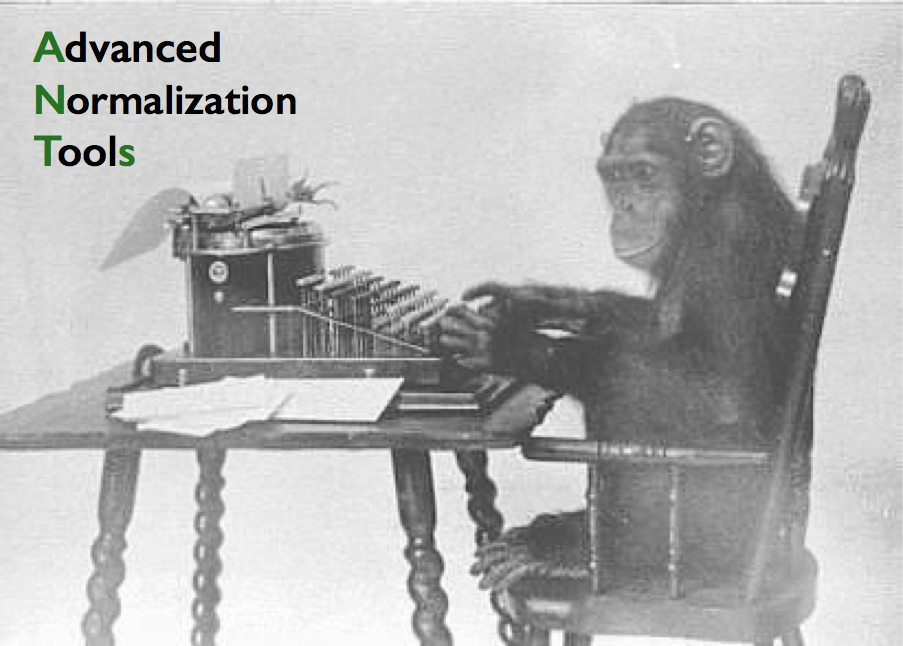
\includegraphics[width=0.45\paperwidth]{./figures/monkeyTypewriter.png}}

\title{Quantitative neuroimaging with ANTs}
\author{Nick Tustison}
\date{}

\begin{document}
\frame{\titlepage}

\section{Background}\label{background}

\begin{frame}{Founding developers}

BBA \& NJT

\end{frame}

\begin{frame}{Long-term collaborators}

\begin{figure}[htbp]
\centering
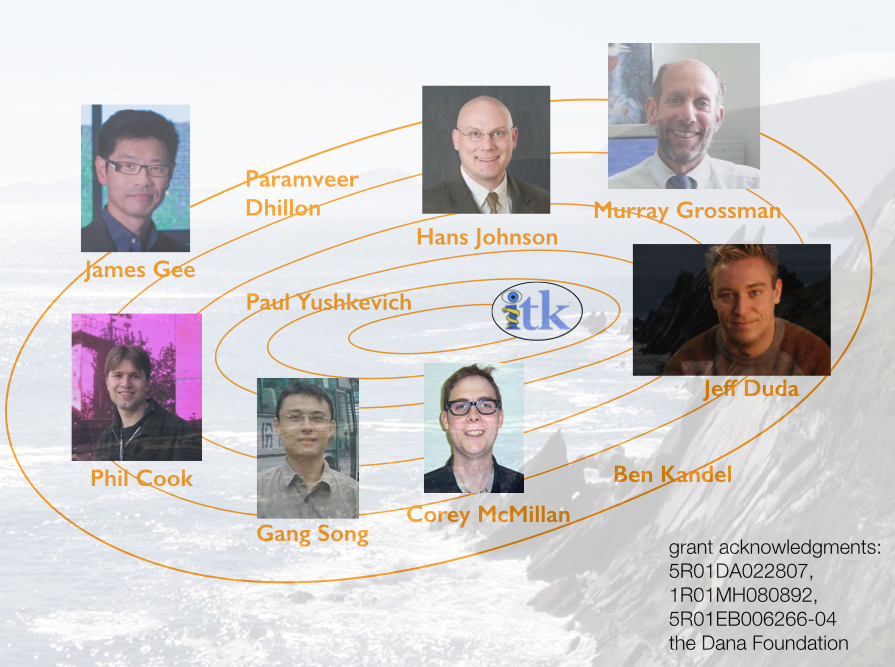
\includegraphics{./figures/antscollab.jpg}
\caption{}
\end{figure}

\(+\) \href{http://neuro.debian.net/pkgs/ants.html}{neurodebian},
\href{http://www.slicer.org/}{slicer},
\href{https://github.com/BRAINSia/BRAINSTools}{brainsfit},
\href{http://nipy.sourceforge.net/nipype/}{nipype},
\href{http://www.itk.org}{itk} and more \ldots{}

\end{frame}

\begin{frame}{}

\begin{figure}[htbp]
\centering
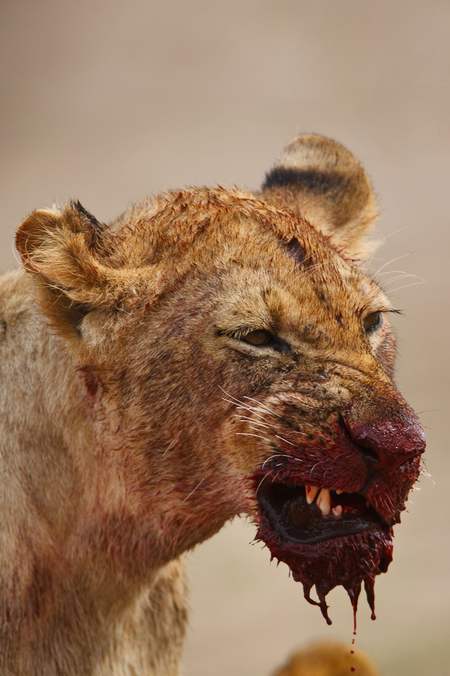
\includegraphics{./figures/lion.png}
\caption{}
\end{figure}

a pride: common way of doing things

\ldots{} in a competitive world \ldots{}

\end{frame}

\begin{frame}{Definitions}

\begin{itemize}
\item
  Registration \(=\) estimate an ``optimal'' geometric mapping between
  image pairs or image sets (e.g.~Affine)
\item
  Similarity \(=\) a function relating one image to another, given a
  transformation (e.g.~mutual information)
\item
  Diffeomorphisms \(=\) differentiable map with differentiable inverse
  (e.g. ``silly putty'', viscous fluid)
\item
  {Segmentation \(=\) labeling tissue or anatomy in images, usually
  automated (e.g.~K-means)}
\item
  Multivariate \(=\) using many voxels or measurements at once
  (e.g.~PCA, \(p >> n\) ridge regression)
\item
  {Multiple modality \(=\) using many modalities at once (e.g.~DTI and
  T1 and BOLD)}
\item
  MALF: multi-atlas label fusion - using anatomical dictionaries to
  label new data
\item
  {Solutions to challenging statistical image processing problems
  usually need elements from each of the above}
\end{itemize}

\end{frame}

\begin{frame}{Image mapping \& perception: 1878}

\begin{figure}[htbp]
\centering
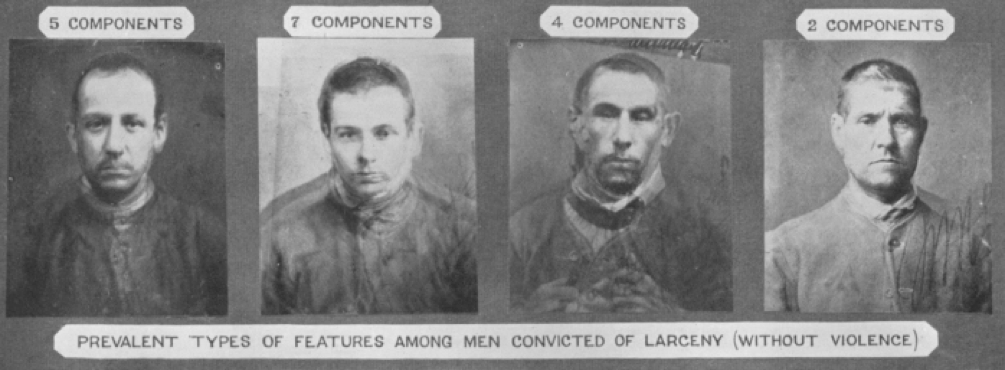
\includegraphics{./figures/galton.png}
\caption{}
\end{figure}

\begin{itemize}
\item
  Francis Galton: Can we see criminality in the face?
\item
  (maybe he should have used \emph{ANTs}?)
\end{itemize}

\end{frame}

\begin{frame}{Image mapping \& biology: 1917}

\begin{figure}[htbp]
\centering
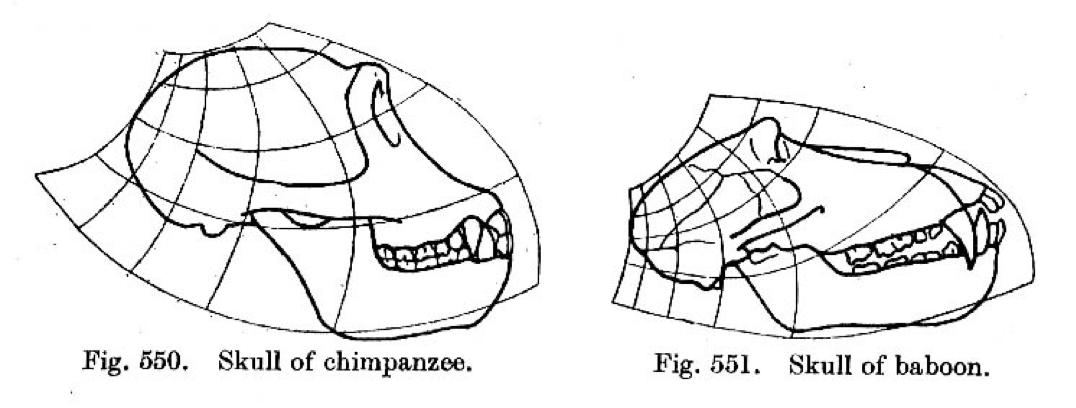
\includegraphics{./figures/dthompson.png}
\caption{}
\end{figure}

D'Arcy Thompson

\end{frame}

\begin{frame}{Initial scope}

\begin{figure}[htbp]
\centering
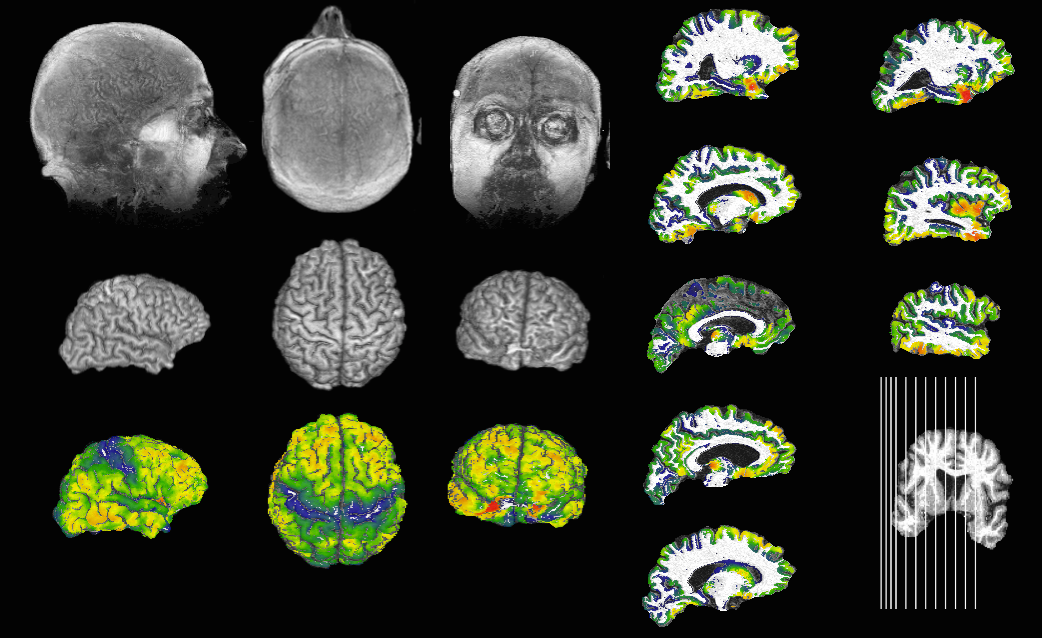
\includegraphics{./figures/ants_initial_scope.png}
\caption{}
\end{figure}

\ldots{} just do a better registration (tell story) \ldots{}

\end{frame}

\begin{frame}{\emph{ANTs} Lineage}

\begin{figure}[htbp]
\centering
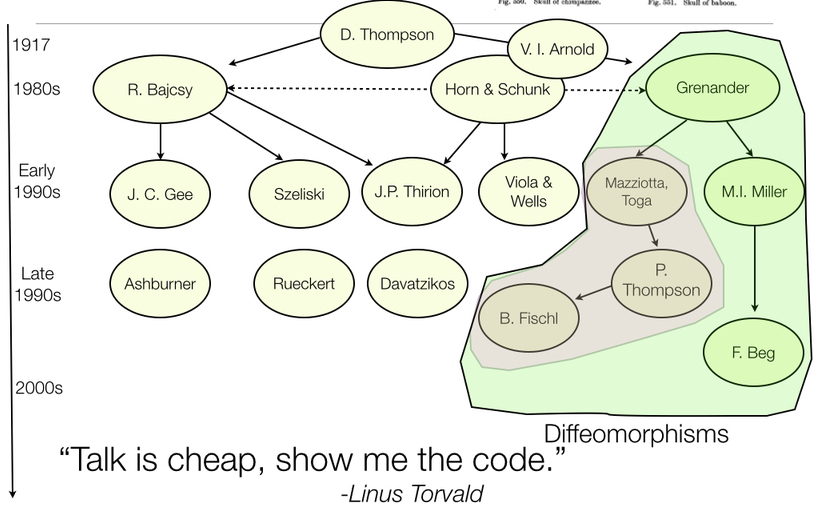
\includegraphics{./figures/lineage.jpg}
\caption{}
\end{figure}

References: Horn and Schunck (1981), Gee, Reivich, and Bajcsy (1993),
Grenander (1993), Thompson et al. (2001), Miller, Trouve, and Younes
(2002), Shen and Davatzikos (2002), Arnold (2014), Thirion (1998),
Rueckert et al. (1999), Fischl (2012), Ashburner (2012)

\end{frame}

\begin{frame}{Diffeomorphisms}

plausible physical modeling of large, invertible deformations

``differentiable map with differentiable inverse''

\end{frame}

\begin{frame}{Fine-grained and flexible maps}

\begin{figure}[htbp]
\centering
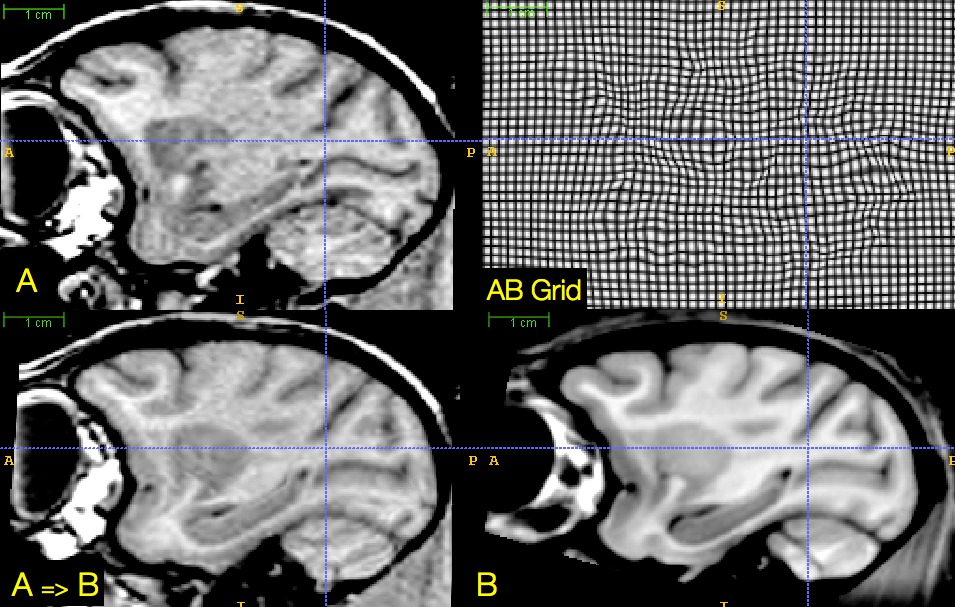
\includegraphics{./figures/highresdiffeos.jpg}
\caption{}
\end{figure}

\ldots{} to correct a misconception about diffeomorphisms \ldots{}

\end{frame}

\begin{frame}{Diffeomorphisms: image parameterization in a metric space}

\begin{figure}[htbp]
\centering
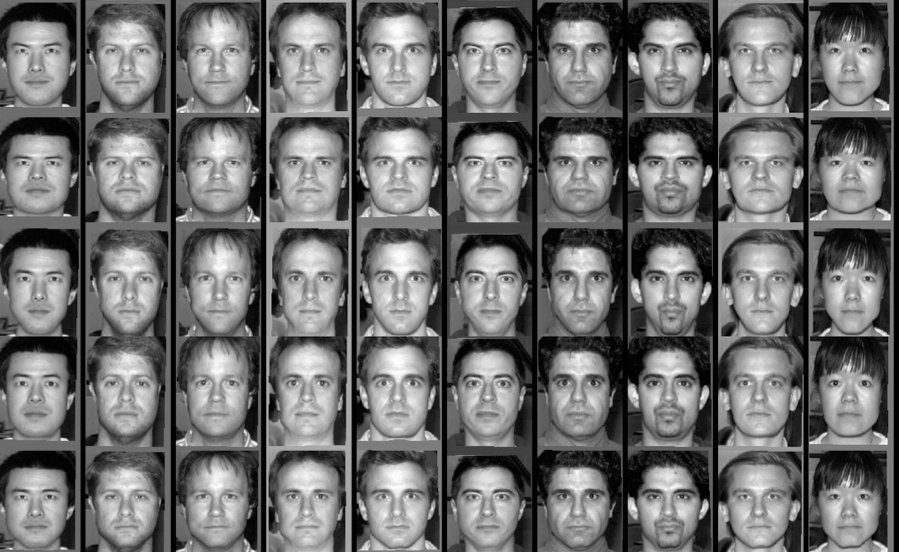
\includegraphics{./figures/shape_appearance.png}
\caption{}
\end{figure}

\end{frame}

\begin{frame}[fragile]{General purpose library for multivariate image
registration, segmentation \& statistical analysis tools}

\begin{itemize}
\item
  170,000+ lines of C++, 6\(+\) years of work, 15+ collaborators.
\item
  Generic mathematical methods that are tunable for application specific
  domains: no-free lunch
\item
  Deep testing on multiple platforms \ldots{} osx, linux, windows.
\item
  Several ``wins'' in public knock-abouts (
  \href{http://www.ncbi.nlm.nih.gov/pubmed/19195496}{Klein 2009},
  \href{http://www.ncbi.nlm.nih.gov/pubmed/21632295}{Murphy 2011},
  \href{http://www.ncbi.nlm.nih.gov/pmc/articles/PMC3837555/}{SATA 2012
  and 2013},
  \href{http://martinos.org/qtim/miccai2013/proc_brats_2013.pdf}{BRATS
  2013}, others )
\end{itemize}

\begin{verbatim}
    An algorithm must use prior knowledge about a problem
    to do well on that problem
\end{verbatim}

\end{frame}

\begin{frame}{\emph{ANTs}: Beyond Registration}

\begin{figure}[htbp]
\centering
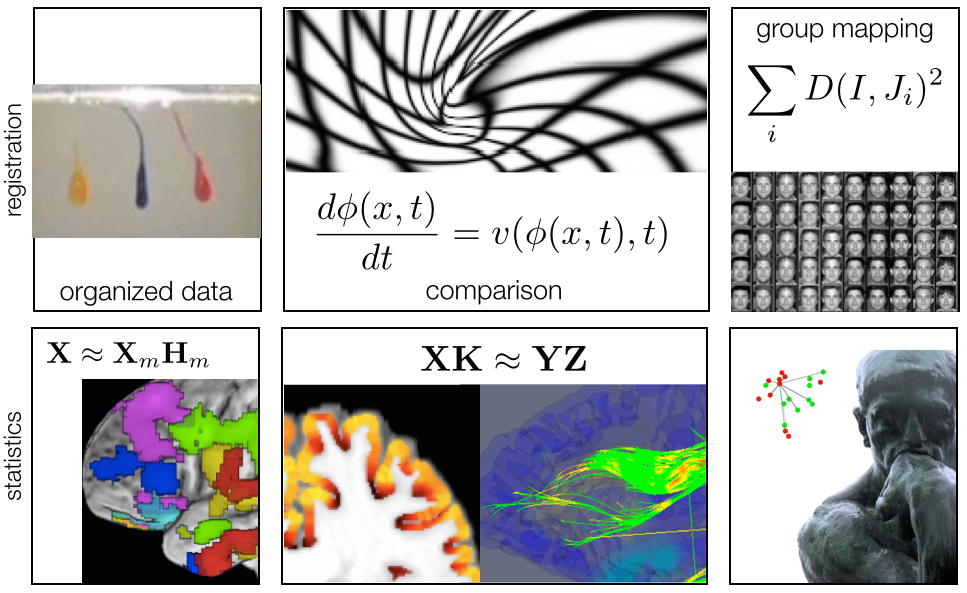
\includegraphics{./figures/antscapabilities.jpg}
\caption{}
\end{figure}

\href{http://www.ncbi.nlm.nih.gov/pubmed/?term=atropos+tustison}{Atropos}
segmentation,
\href{http://www.ncbi.nlm.nih.gov/pubmed/?term=N4+tustison}{N4
inhomogeneity correction},
\href{http://www.ncbi.nlm.nih.gov/pubmed/?term=eigenanatomy+avants}{Eigenanatomy},
\href{http://www.ncbi.nlm.nih.gov/pubmed/?term=sparse+canonical+avants}{SCCAN},
\href{http://www.ncbi.nlm.nih.gov/pubmed/24852460}{Prior-constrained
PCA}, and
\href{http://www.ncbi.nlm.nih.gov/pmc/articles/PMC4009425/}{atlas-based
label fusion} and
\href{http://www.ncbi.nlm.nih.gov/pubmed/21237273}{MALF} (powerful
expert systems for segmentation)

\end{frame}

\begin{frame}{On documentation}

\begin{figure}[htbp]
\centering
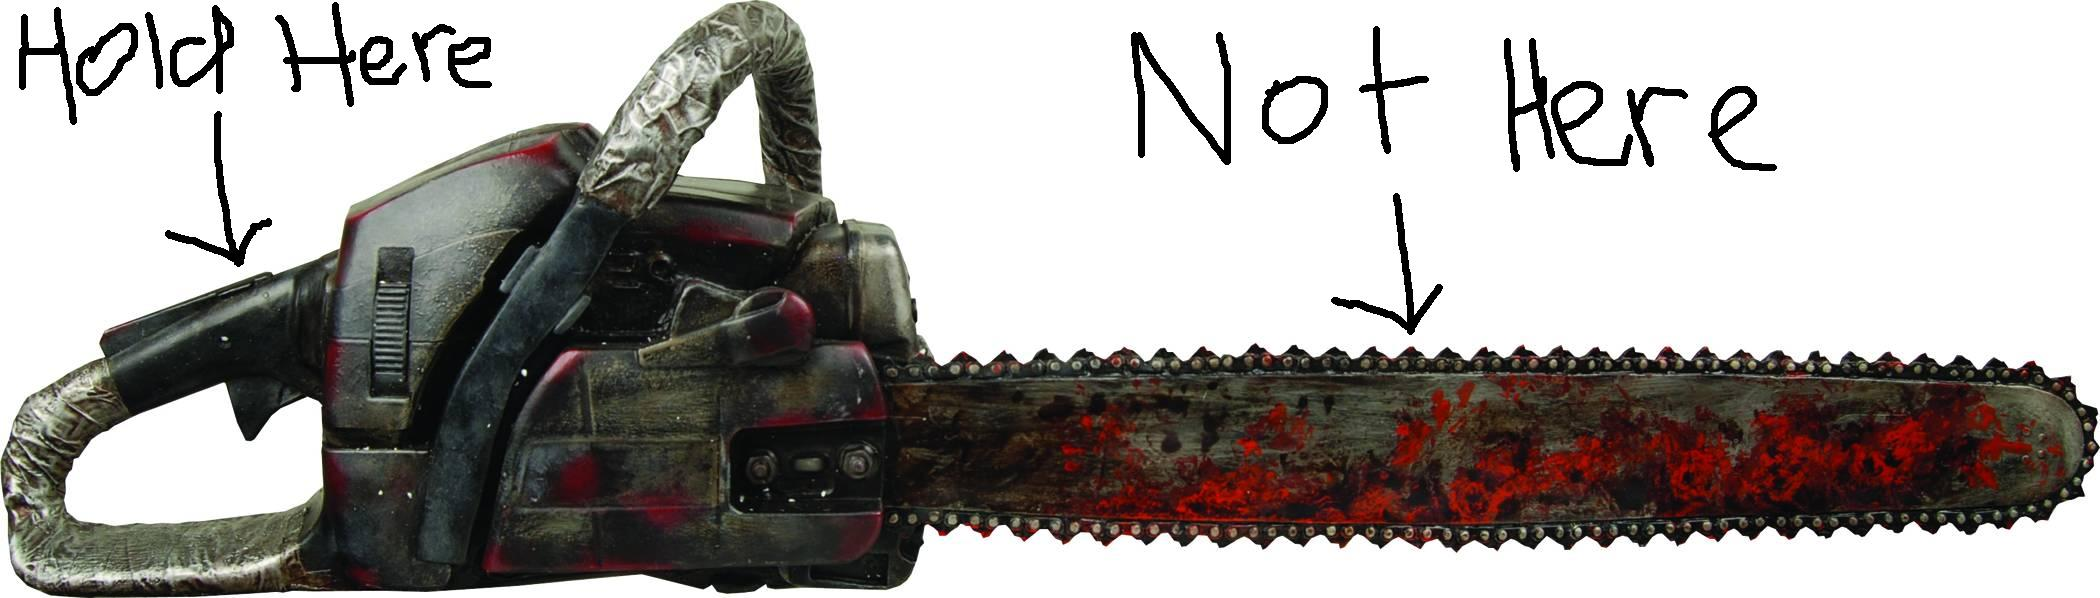
\includegraphics{figures/Chainsaw.jpg}
\caption{}
\end{figure}

documentation is important

\end{frame}

\begin{frame}{On documentation}

\begin{figure}[htbp]
\centering
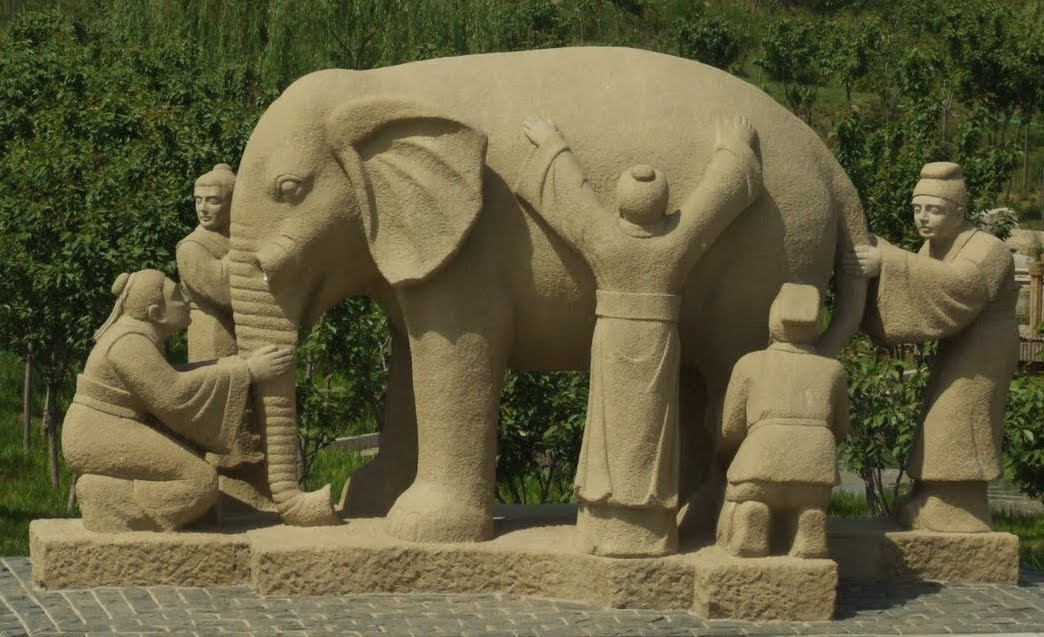
\includegraphics{figures/blindmen.jpg}
\caption{}
\end{figure}

\ldots{} developers can be blind to doc deficiencies

while users are blind to what we provide!

\hypertarget{refs}{}
\hypertarget{ref-Arnold2014}{}
Arnold, Vladimir I. 2014. ``Topological Methods in Hydrodynamics.'' In
\emph{Vladimir I. Arnold-Collected Works}, 433--54. Springer.
\url{http://link.springer.com/chapter/10.1007/978-3-642-31031-7_42}.

\hypertarget{ref-Ashburner2012}{}
Ashburner, John. 2012. ``SPM: A History.'' \emph{Neuroimage} 62 (2).
Wellcome Trust Centre for Neuroimaging, 12 Queen Square, London WC1N
3BG, UK. john@fil.ion.ucl.ac.uk: 791--800.
doi:\href{https://doi.org/10.1016/j.neuroimage.2011.10.025}{10.1016/j.neuroimage.2011.10.025}.

\hypertarget{ref-Fischl2012}{}
Fischl, Bruce. 2012. ``FreeSurfer.'' \emph{Neuroimage} 62 (2). Athinoula
A Martinos Center, Dept. of Radiology, MGH, Harvard Medical School, MA
fischl@nmr.mgh.harvard.edu, USA. fischl@nmr.mgh.harvard.edu: 774--81.
doi:\href{https://doi.org/10.1016/j.neuroimage.2012.01.021}{10.1016/j.neuroimage.2012.01.021}.

\hypertarget{ref-Gee1993}{}
Gee, J. C., M. Reivich, and R. Bajcsy. 1993. ``Elastically Deforming 3D
Atlas to Match Anatomical Brain Images.'' \emph{J Comput Assist Tomogr}
17 (2). Department of Computer; Information Science, University of
Pennsylvania, Philadelphia 19104.: 225--36.

\hypertarget{ref-Grenander1993}{}
Grenander, Ulf. 1993. \emph{General Pattern Theory-a Mathematical Study
of Regular Structures}. Clarendon Press.

\hypertarget{ref-Horn1981}{}
Horn, Berthold K, and Brian G Schunck. 1981. ``Determining Optical
Flow.'' In \emph{1981 Technical Symposium East}, 319--31. International
Society for Optics; Photonics.
\url{http://proceedings.spiedigitallibrary.org/proceeding.aspx?articleid=1231385}.

\hypertarget{ref-Miller2002}{}
Miller, Michael I., Alain Trouve, and Laurent Younes. 2002. ``On the
Metrics and Euler-Lagrange Equations of Computational Anatomy.''
\emph{Annu Rev Biomed Eng} 4. Center for Imaging Science, The Johns
Hopkins University, Baltimore, Maryland 21218, USA. mim@cis.jhu.edu:
375--405.
doi:\href{https://doi.org/10.1146/annurev.bioeng.4.092101.125733}{10.1146/annurev.bioeng.4.092101.125733}.

\hypertarget{ref-Rueckert1999}{}
Rueckert, D., L. I. Sonoda, C. Hayes, D. L. Hill, M. O. Leach, and D. J.
Hawkes. 1999. ``Nonrigid Registration Using Free-Form Deformations:
Application to Breast MR Images.'' \emph{IEEE Trans Med Imaging} 18 (8).
Division of Radiological Sciences; Medical Engineering, Guy's, King's,;
St. Thomas' School of Medicine, King's College London, Guy's Hospital,
London, UK. D.Rueckert@umds.ac.uk: 712--21.
doi:\href{https://doi.org/10.1109/42.796284}{10.1109/42.796284}.

\hypertarget{ref-Shen2002}{}
Shen, Dinggang, and Christos Davatzikos. 2002. ``HAMMER: Hierarchical
Attribute Matching Mechanism for Elastic Registration.'' \emph{IEEE
Trans Med Imaging} 21 (11). Center for Biomedical Image Computing,
Department of Radiology, The Johns Hopkins University School of
Medicine, 601 N. Caroline Street, Baltimore, MD 21287, USA.
dgshen@rad.upenn.edu: 1421--39.
doi:\href{https://doi.org/10.1109/TMI.2002.803111}{10.1109/TMI.2002.803111}.

\hypertarget{ref-Thirion1998}{}
Thirion, J. P. 1998. ``Image Matching as a Diffusion Process: An Analogy
with Maxwell's Demons.'' \emph{Med Image Anal} 2 (3). INRIA, Equipe
Epidaure, Sophia-Antipolis, France. jean-philippe.thirion@inria.fr:
243--60.

\hypertarget{ref-Thompson2001}{}
Thompson, Paul M., Michael S. Mega, Christine Vidal, Judith L. Rapoport,
and Arthur W. Toga. 2001. ``Detecting Disease-Specific Patterns of Brain
Structure Using Cortical Pattern Matching and a Population-Based
Probabilistic Brain Atlas.'' \emph{Inf Process Med Imaging} 2082.
Laboratory of Neuro Imaging, Division of Brain Mapping,; Alzheimer's
Disease Center, Dept. of Neurology, UCLA School of Medicine, Los
Angeles, CA, USA thompson@loni.ucla.edu.: 488--501.
doi:\href{https://doi.org/10.1007/3-540-45729-1_52}{10.1007/3-540-45729-1\_52}.

\end{frame}

\end{document}
